\documentclass[12pt]{article}
\usepackage{color}
\usepackage{floatrow}
\usepackage[margin=1in]{geometry}
\usepackage{listings}
\usepackage{setspace}
\usepackage{tikz}
\usepackage{graphicx}
\usepackage{subfig}
\usepackage{amsmath}
\usepackage{gnuplottex}

\usepackage{hyperref}
\hypersetup{
    colorlinks=true,
    linkcolor=black,
    filecolor=magenta,      
    urlcolor=black,
}

\definecolor{dkgreen}{rgb}{0,0.6,0}
\definecolor{gray}{rgb}{0.5,0.5,0.5}
\definecolor{mauve}{rgb}{0.58,0,0.82}

\usepackage{pgfplots}
\pgfplotsset{width=10cm,compat=1.9}
\pgfplotsset{scaled y ticks=false}

\setstretch{1}
\graphicspath{{images}}

\edef\restoreparindent{\parindent=\the\parindent\relax}
\usepackage{parskip}
\restoreparindent

\lstset{
  frame=tb,
  language=C++,
  aboveskip=3mm,
  belowskip=3mm,
  showstringspaces=false,
  columns=flexible,
  basicstyle={\small\ttfamily},
  numbers=none,
  numberstyle=\tiny\color{gray},
  keywordstyle=\color{blue},
  commentstyle=\color{dkgreen},
  stringstyle=\color{mauve},
  breaklines=true,
  breakatwhitespace=true,
  tabsize=3
}

\title{Mathematical Approach to an Optimal Algorithmic \textit{Snake} Game Agent}
\author{hxl941}
\date{April 12, 2021}

\begin{document}
\begin{singlespace}
\maketitle
\thispagestyle{empty}
\tableofcontents
\end{singlespace}

\clearpage
\setcounter{page}{1}
\pagebreak


\section{Introduction}

A primary focus of mathematics is modelling and optimizing real-life scenarios to automate processes or maximize desired results while minimizing use of resources. This field has countless practical applications in the realms of scientific and algorithmic problems.

As an aspiring computer scientist, I have developed a particular interest in the intersection between math and programming. Alongside my passion for applied math, I also enjoy playing video games, being introduced to them after I first played the popular \textit{Snake} game on an old Nokia 3310 during my childhood. After taking the HL Math course, I started thinking about the things I regularly do from a mathematical perspective, so naturally, I decided to find a mathematically suitable way to create an efficient and autonomous agent for the \textit{Snake} game.

Hence, this investigation aims to find various \textbf{mathematical approaches to creating an optimal algorithmic \textit{Snake} game agent} and comparing them to conclusively determine the most efficient solution. For this investigation the most efficient algorithm will be the one which beats the game in the minimum amount of time. All approaches will be transformed into software agents for testing. This exploration will look at graph theory as a way to model the game and arrive at raw base approaches which will then be evaluated and combined with an analytical approach using probability density functions and calculus. 

\section{\textit{Snake} Game Mechanics}

In my implementation of the \textit{Snake} game (Figure \ref{fig:game_mechanics}), the autonomous agent controls a snake on the game plane. As the snake moves forward, left or right, it leaves a trail of fixed size behind it. The snake grows longer when its head runs into the apples and dies when it runs into itself or the borders. The objective is to grow long enough to cover the grid entirely, at which point the game is won.

\begin{figure}[!h]
\centering
\floatbox[{\capbeside\thisfloatsetup{capbesideposition={right,center},capbesidewidth=8cm}}]{figure}[\FBwidth]
	{\caption{The graphical representation of my implementation of the \textit{Snake} game. The \texttt{\makeatletter @\makeatother}, \texttt{\#} and red digit represent the snake's head, the snake's body and the apple, respectively} \label{fig:game_mechanics}
}
	{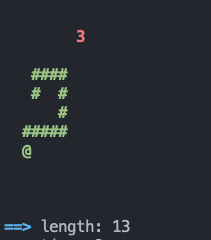
\includegraphics[scale=0.6]{game_mechanics.png}}
\end{figure}

\section{Modelling The Game}

While researching suitable models for representing the game, I came across graph theory, which is a branch in discrete mathematics. Although this was not taught in class, I found many explanatory articles online.

\subsection{Graph Theory}

Graph theory refers to a way in which data can be represented. A graph is a pair $G=(V,E)$ where $V$ is a set of vertices and $E$ is a set of pairs of vertices. The edge $e$ between vertices $v_{1}$ and $v_{2}$ is written as $e=v_{1}v_{2}$. $v_{1}$ and $v_{2}$ are thus the endpoints of edge $e$ and are said to be adjacent to each other \cite{galvin2009}. A pair of vertices can be joined by at most one edge and no vertex can be joined to itself by an edge. For example, $G_{1}=(V_{1},E_{1})$ where $V_{1}=\{v_{1}, v_{2}, v_{3}\}$ and $E_{1}=\{v_{1}v_{2}, v_{2}v_{3}\}$ is drawn:

\begin{figure}[!h]
\centering
	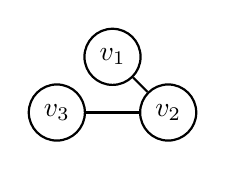
\begin{tikzpicture}[node distance={10mm}, main/.style={draw,circle}, thick]
		\node[main] (1) {$v_{1}$};
		\node[main] (2) [below right of=1] {$v_{2}$};
		\node[main] (3) [below left of=1] {$v_{3}$};

		\draw (1) to (2);
		\draw (2) to (3);
	\end{tikzpicture}
	\caption{Graph $G_{1}$}
	\label{fig:graph_g1}
\end{figure}

In graphs, there sometimes exist paths between two vertices and cycles containing multiple vertices. Formally, a graph $G_{p}=(V_{p}, E_{p})$ of $n$ vertices is a path from vertex $v_{1}$ to $v_{n}$ if $V_{p} = \{v_{1}, \ldots , v_{n} \}$ and $E_{p} = \{v_{i}v_{i+1} | i = 1, \ldots, n - 1\}$ \cite{galvin2009}. $G_{p}$ is a cycle under the condition that $E_{p} = \{v_{i}v_{i+1} | i = 1, \ldots, n - 1\} \cup \{ v_{n}v_{1} \}$ \cite{galvin2009}.

\subsection{Representing \textit{Snake} As A Graph}

To represent \textit{Snake} as a graph, it must first be visualized as a grid of width $m$ and height $n$ with $mn$ cells where each cell $c$ has coordinates $\{ (x, y) | 1 \leq x \leq m, 1 \leq y \leq n \}$ and the cell $c=(1,1)$ is at the first row of the first column of the grid (see Figure \ref{fig:snake_grid}).

\begin{figure}[!h]
\centering
	\begin{tabular}{ | c | c | c | }
	\hline
	$(1, 1)$ & \ldots & $(m, 1)$ \\
	\hline
	\ldots &  & \ldots \\
	\hline
	$(1, n)$ & \ldots & $(m, n)$ \\
	\hline		
	\end{tabular}
	\caption{The \textit{Snake} game plane in grid format}
	\label{fig:snake_grid}
\end{figure}

Under this model, the position of the snake and the apple can be represented as a set of cells and an individual cell, respectively. The snake can travel to cells that are adjacent to its head and are not already occupied by itself. To express this model as graph $G=(V,E)$ (see Figure \ref{fig:graph_g}), we make the following considerations:

\begin{enumerate}
	\item Each cell $c$ can be represented as some vertex $v=\{(c_{x}, c_{y}) | 1 \leq c_{x} \leq m, 1 \leq c_{y} \leq n \}$. The set of vertices $V$ can thus be represented as $V=\{v_{i,j} | 1 \leq i \leq m, 1 \leq j \leq n \}$ where vertex $v_{i,j}$ refers to the cell at coordinates $(i,j)$.
	\item In the grid, the snake can travel to each cell non-diagonally adjacent to its head. We can express the ability to travel from one cell to another as an edge between the corresponding two vertices. Therefore, for all $v_{i,j} \in V$, there exists an edge to $v_{i+1,j}$, $v_{i-1,j}$, $v_{i,j+1}$ and $v_{i,j-1}$ in $E$ if these adjacent vertices are in $V$.
	\item The snake's body can be represented as a set of vertices $S$ containing the vertices occupied by the snake's body such that $S \subseteq V$.
	\item The snake head can be represented as some vertex $v_{i,j} \in V$, denoted $v_{h}$ for presentation.
	\item The apple can be represented as some vertex $v_{i,j} \in V$, denoted $v_{a}$ for presentation.
\end{enumerate}

\begin{figure}[!h]
\centering
	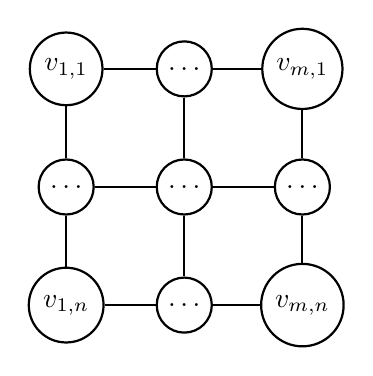
\begin{tikzpicture}[node distance={15mm}, main/.style={draw,circle}, thick]
		\node[main] (1) {$v_{1,1}$};
		\node[main] (2) [right of=1] {$\ldots$};
		\node[main] (3) [right of=2] {$v_{m,1}$};
		\node[main] (4) [below of=1] {$\ldots$};
		\node[main] (5) [below of=2] {$\ldots$};
		\node[main] (6) [below of=3] {$\ldots$};
		\node[main] (7) [below of=4] {$v_{1,n}$};
		\node[main] (8) [right of=7] {$\ldots$};
		\node[main] (9) [below of=6] {$v_{m,n}$};


		\draw (1) to (2);
		\draw (1) to (4);
		\draw (2) to (3);
		\draw (3) to (6);
		\draw (4) to (7);
		\draw (4) to (5);
		\draw (2) to (5);
		\draw (5) to (8);
		\draw (5) to (6);
		\draw (6) to (9);
		\draw (7) to (8);
		\draw (8) to (9);
	\end{tikzpicture}
	\caption{Graph $G$}
	\label{fig:graph_g}
\end{figure}

\section{Base Approaches}

This model represents the current state and the positions of the snake and the apple on the game plane. The end goal is to be able to program a mathematical approach; a common way to implement mathematical logic into computer programs is to describe it in a function where the current state is passed as input and a useful value is returned.

For this exploration, this function must find the best path that the snake should follow to win the game. With this path generated, the first edge in the set of edges of the path contains the next vertex of where the snake head needs to be. Knowing this, the program can calculate the direction in which the snake must turn. Therefore, the return value should be the first edge of the best path.

\subsection{Breadth-First Search}

An intuitive method for generating the best path with the goal of producing a time efficient solution is to compute the shortest path between the snake head and the apple since it is the quickest way for the snake to reach the apple and increase in size. A systematic approach for finding the shortest path between two vertices in a graph is to use the Breadth-First Search (BFS) algorithm. In the real-world, alongside other path-finding algorithms such as A-star and Dijkstra's, BFS is used in problems where exploring a graph is needed, such as for finding optimal flight routes between two cities. The BFS traversal of a graph terminates when every vertex of the graph has been visited. The concept is to visit all adjacent vertices of the starting vertex before visiting the vertices adjacent to the adjacent vertices. The algorithm takes the following steps \cite{gadagkar2019}:

\begin{enumerate}
	\item Keep a list of all vertices seen so far. Add the starting vertex to this list.
	\item Take the first vertex from the list, visit it and add unvisited adjacent vertices to the end of the list.
	\item Repeat the previous step until the list is empty.
\end{enumerate}

Consider Figure \ref{fig:graph_g2} with graph $G_{2} = (V_{2}, E_{2})$:

\begin{figure}[!h]
\centering
	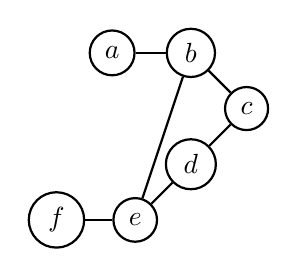
\begin{tikzpicture}[node distance={10mm}, main/.style={draw,circle}, thick]
		\node[main] (1) {$a$};
		\node[main] (2) [right of=1] {$b$};
		\node[main] (3) [below right of=2] {$c$};
		\node[main] (4) [below left of=3] {$d$};
		\node[main] (5) [below left of=4] {$e$};
		\node[main] (6) [left of=5] {$f$};

		\draw (1) to (2);
		\draw (2) to (3);
		\draw (3) to (4);
		\draw (2) to (5);
		\draw (4) to (5);
		\draw (5) to (6);
	\end{tikzpicture}
	\caption{Graph $G_{2}$}
	\label{fig:graph_g2}
\end{figure}

Directly applying the BFS algorithm with starting vertex $a$, the traversal for the graph $G_{2}$ would be: $a \rightarrow b \rightarrow c \rightarrow e \rightarrow d \rightarrow f$. Rather than traversing all vertices, the application of BFS for the \textit{Snake} game problem requires finding the shortest path between the snake head and the apple. To accomplish this goal, we can modify the initial algorithm as such \cite{bose_howat2015}:

\begin{enumerate}
	\item Keep a list of vertices seen so far and the path required to get to the vertex as a pair. Add the pair of the starting vertex and an empty path to this list.
	\item Take the first pair from the list. This pair will have vertex $v$ and path $P$. Visit $v$ and for each unvisited vertex $u$ adjacent to $v$, duplicate path $P$ but also add edge $e = vu$ to it and finally add the pair $(u, \textrm{modified path } P)$ to the end of the list.
	\item Repeat the previous step until the end vertex is added to the list, in which case the associated path will be the shortest path from the starting vertex to the end vertex and return this path. In the case that the list is empty, return an empty path.
\end{enumerate}

Applying this modified BFS algorithm to $G_{2} $ with starting vertex $a$ and end vertex $e$, we see that the edges of the generated path are correctly $\{ab, be\}$ rather than $\{ab, bc, cd, de\}$. Therefore, this algorithm is suitable for finding the aforementioned best path for the snake to take under the shortest path approach.

To apply BFS to the \textit{Snake} game, we set $v_{h}$ as the starting vertex and $v_{a}$ as the end vertex. One final modification to make, to ensure that the generated path does not involve the snake head running into its body, is to add the following rule to step 2 from the modified algorithm: only adjacent vertices $u$ that are not already occupied by the snake's body should be added to the list. The final code for this approach is shown in Figure \ref{fig:bfs_code} of Appendix \ref{sec:appendix_code}.

Despite being a very quick solution and seemingly sound at first glance, a more comprehensive examination of the shortest path approach reveals a major flaw. Since the BFS algorithm is a greedy solution to the problem, in that it finds the best move for the current state and performs it without thinking of the consequences, it is not able to foresee the position of the snake after it has moved along the shortest path and thus traps itself. After running 10 000 simulations with this approach, it was never successful at beating the game. Each game ends in the ways shown in Figure \ref{fig:bfs_issues}.

\begin{figure}[!h]
\centering
	\subfloat[The apple gets enclosed by the snake]{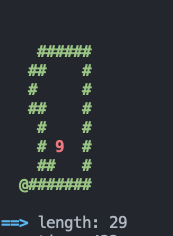
\includegraphics[scale=0.6]{circled_apple.png}\label{fig:bfs_issues_apple}}
	\hspace{1.15em}
	\subfloat[The snake traps itself along the border]{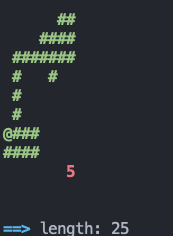
\includegraphics[scale=0.6]{circled_self.png}\label{fig:bfs_issues_self}}
	\caption{Losing scenarios with the BFS approach}
	\label{fig:bfs_issues}
\end{figure}

\subsection{Hamiltonian Cycle}

To remedy the flaw in the BFS approach, I decided to focus on a solution that would guarantee a win even if it meant that it might not be efficient time-wise. In my research, I watched videos of players winning \textit{Snake}. At first these players would take a greedy shortest path approach but changed their strategy once the snake got longer, instead looping one fixed cycle \cite{easyspeezy2020}. They traverse the game plane such that they visit each point exactly once before returning to the starting point. This is recognized as a Hamiltonian cycle, formally defined to be a closed loop on a graph where each vertex is visited exactly once \cite{rahman2005}. Consider Figure \ref{fig:graph_g3} with graph $G_{3} = (V_{3}, E_{3})$:

\begin{figure}[!h]
\centering
	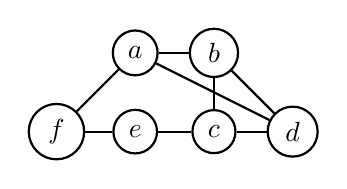
\begin{tikzpicture}[node distance={10mm}, main/.style={draw,circle}, thick]
		\node[main] (1) {$a$};
		\node[main] (2) [right of=1] {$b$};
		\node[main] (3) [below of=2] {$c$};
		\node[main] (4) [right of=3] {$d$};
		\node[main] (5) [below of=1] {$e$};
		\node[main] (6) [left of=5] {$f$};

		\draw (1) to (2);
		\draw (1) to (6);
		\draw (2) to (3);
		\draw (3) to (4);
		\draw (1) to (4);
		\draw (2) to (4);
		\draw (3) to (5);
		\draw (5) to (6);
	\end{tikzpicture}
	\caption{Graph $G_{3}$}
	\label{fig:graph_g3}
\end{figure}

$G_{3}$ is said to be Hamiltonian since there is a Hamiltonian cycle: $a \rightarrow b \rightarrow d \rightarrow c \rightarrow e \rightarrow f \rightarrow a$. The rationale behind having the snake follow this cycle is that it will never be trapped since it will not be able to run into itself until the entire graph consists only of the snake. Thus, it is guaranteed that an agent based on this approach will win the game.

For graph $G$ to be Hamiltonian, its width $m$ and height $n$ must follow these constraints:

\begin{itemize}
	\item $m>1$, $n>1$ and either $m$ or $n$ is even. \textbf{Proof by construction} \cite{zagaran2018}: If $m$ or $n$ is 2, a Hamiltonian cycle can be constructed by forming a ring around the vertices. Otherwise, there must be a side in the grid with an even number of vertices greater than 2. We will call this direction \textit{vertical} (meaning that the graph will have an even number of rows) and the other direction \textit{horizontal}. Start from the first column of the first row and begin the path by extending it to the last column of this first row. Go one row below and return to the second column. If this is the last row of the graph, then extend the path to the first column and connect it back to the vertex on the first column of the first row. If this is not the last row, then stay on the second column, drop one column down and repeat the initial process. Since there are an even number of rows, there will be exactly $\frac{n}{2}$ repetitions. Note that if $m > 2$, the length of $m$ does not matter.

Therefore, it is always possible to construct a Hamiltonian cycle when $m>1$, $n>1$ and either $m$ or $n$ is even. See Figure \ref{fig:cycle_proof} for a visual example of the above proof.

\begin{figure}[!h]
\centering
	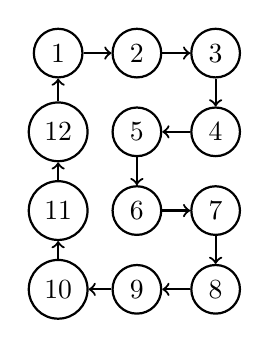
\begin{tikzpicture}[node distance={10mm}, main/.style={draw,circle}, thick]
		\node[main] (1) {1};
		\node[main] (2) [right of=1] {2};
		\node[main] (3) [right of=2] {3};
		\node[main] (4) [below of=3] {4};
		\node[main] (5) [left of=4] {5};
		\node[main] (6) [left of=5] {12};
		\node[main] (7) [below of=6] {11};
		\node[main] (8) [right of=7] {6};
		\node[main] (9) [right of=8] {7};
		\node[main] (10) [below of=9] {8};
		\node[main] (11) [left of=10] {9};
		\node[main] (12) [left of=11] {10};

		\draw[->] (1) to (2);
		\draw[->] (2) to (3);
		\draw[->] (3) to (4);
		\draw[->] (4) to (5);
		\draw[->] (5) to (8);
		\draw[->] (8) to (9);
		\draw[->] (9) to (10);
		\draw[->] (10) to (11);
		\draw[->] (11) to (12);
		\draw[->] (12) to (7);
		\draw[->] (7) to (6);
		\draw[->] (6) to (1);
		
	\end{tikzpicture}
	\caption{Numbered Hamiltonian cycle of grid graph for $m=3$ and $n=4$}
	\label{fig:cycle_proof}
\end{figure}

	
	\item \textbf{Or} $mn = 1$. Under this scenario, the graph contains only one vertex and is trivially Hamiltonian with a zero length cycle that visits the vertex.
\end{itemize}

If only one of $m$ and $n$ are equal to 1, then the graph is a straight line. In this case, it is impossible to form a Hamiltonian cycle. If both $m$ and $n$ are odd and $mn$ is not equal to 1, then we have a bipartite graph with unbalanced vertex parity, which, by Grinberg's Theorem, is known to not be Hamiltonian \cite{zagaran2018}.

To implement this idea in code as an autonomous agent, the most efficient solution would be to generate a Hamiltonian cycle for the game graph when the game is first initialized. This way, the function into which the game state would be the input already has the best path for the snake in memory and the code can check where the snake head is to determine where it should turn next.

Note that generating a Hamiltonian cycle is an NP (non-polynomial time) hard problem in computation, since there are $\frac{1}{2} (n-1)!$ candidate cycles in any graph with $n$ vertices \cite{mitchell2019}. Instead, I used a heuristic proposed by Chuyang Liu \cite{liu2019} (see code in Figure \ref{fig:cycle_code} of Appendix \ref{sec:appendix_code}). After making this implementation, the game can now be won as can be seen in Figure \ref{fig:finished_cycle}.

\begin{figure}[!h]
\centering
	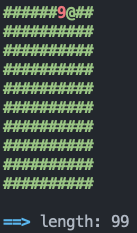
\includegraphics[scale=0.6]{finished_cycle.png}
	\caption{Completed game for a $10 \times 10$ grid}
	\label{fig:finished_cycle}
\end{figure}

While this is a valid approach to solving the game, it does not address the needs outlined in the aim of this investigation of developing an \textbf{optimal} approach: one requiring a minimum amount of time. At the beginning of the game, when the length of the snake is only one, the snake head may need to move up to $mn - 1$ turns before reaching the apple in the worst case scenario. On average, at length $l$, the snake needs to move for $\frac{1}{2} (mn-l)$ turns before reaching the apple. Therefore, this is an extremely slow approach and is thus not the ideal way to mathematically solve the game.

\section{Analytical Approach}

Despite their shortcomings, both the BFS and Hamiltonian cycle approaches had their strengths. For a grid where $m=n=10$, the agent using the BFS approach usually survived until the length of the snake was over 20. Notably, it got to this length very quickly using its greedy shortest path approach. The Hamiltonian cycle on the other hand, despite being a slower approach, always guaranteed that the game would be won.

Referring back to the method that human players took to beat the game, we can observe that a combination of the two aforementioned base approaches will be the most optimal. A final approach, in which both of these solutions are combined, will be enhanced by both of their benefits. To model the human players, the third approach will first begin with BFS followed by a conversion to the Hamiltonian cycle after some length. The most critical aspect with this approach is to determine what length maximizes the benefits of the speed of BFS in order to minimize the time but also assures survival of the snake. To find this length, I can optimize using differential calculus a function $T$  where $T(l_{s})$ represents the total amount of moves (which are to be understood as turns including going straight) that will be taken if the model switches from BFS to the Hamiltonian cycle at length $l_{s}$. Note that much of this analysis requires knowing the size of the grid beforehand. Therefore, $m=n=10$ will be used as the grid size for the game plane.

\subsection{Modelling Each Approach}

The first step to take is to model each of the two base approaches with respect to the average amount of moves required for increasing the length to $l+1$ when the snake is at length $l$.

For the BFS approach, I found this relationship experimentally by letting a BFS agent play the game 10 000 times. For each game, I added a data point of how many moves it took for a snake of length $l$ to get to $l+1$, and then averaged this data. The results are summarized in the graph below (see Figure \ref{fig:bfs_sim_data}).

The limited domain of the data points collected is a result of the fact that with the BFS agent, the snake begins dying a lot more often as the snake length increases (since it is more likely to trap itself), so only this domain was deemed applicable for analysis. In order to express this relationship as a function, I considered the use of several different trend line models for the scatter plot. However, I noted that a polynomial function could not be used given that it must extrapolate the number of moves required over the entire available domain with respect to the maximum snake length of 99. In a polynomial function, the end behaviours would govern the extrapolation for larger snake lengths beyond $l=27$.

\begin{figure}[!h]
\centering
	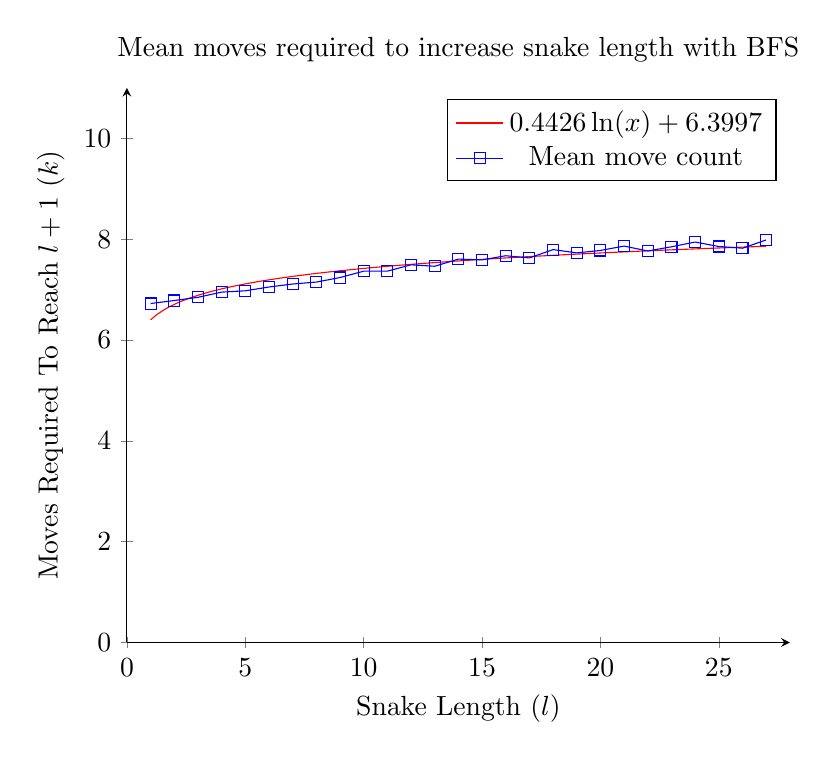
\begin{tikzpicture}
		\begin{axis}[
			title={Mean moves required to increase snake length with BFS},
		    axis lines = left,
		    xlabel = {Snake Length ($l$)},
    		ylabel = {Moves Required To Reach $l+1$ ($k$)},
    		xmin=0, xmax=28,
		    ymin=0, ymax=11,
		]

			\addplot [
		    	domain=1:27, 
	    		samples=100, 
		    	color=red,
			]
			{0.4426*ln(x) + 6.3997};
			\addlegendentry{$0.4426\ln(x) + 6.3997$}
			
			\addplot[
   				color=blue,
    			mark=square,
		    ]
		    coordinates {(1,6.7229)
(2,6.7823)
(3,6.8457)
(4,6.9491)
(5,6.9752)
(6,7.0507)
(7,7.1095)
(8,7.1485)
(9,7.2382)
(10,7.3644)
(11,7.3646)
(12,7.4905)
(13,7.462)
(14,7.6039)
(15,7.5882)
(16,7.6704)
(17,7.6272)
(18,7.7923)
(19,7.7273)
(20,7.7751)
(21,7.8624)
(22,7.7648)
(23,7.8479)
(24,7.9422)
(25,7.8537)
(26,7.8199)
(27,7.9838)};
  		   \addlegendentry{Mean move count}
		\end{axis}
	\end{tikzpicture}
	\caption{}
	\label{fig:bfs_sim_data}
\end{figure}

Therefore, observing that the graphed data points on the scatter plot appeared to be shaped concave down, I decided to use a logarithmic function to model the relationship. The corresponding trend line equation was computed in Microsoft Excel. Calculating Pearson's coefficient value to determine the validity of this model, the result is $R^2 = 0.9358$, indicating that this equation is a good fit. This is a logically suitable model, since the length of the shortest path should increase when more vertices are blocked by the snake body. Let $b(l)$ be the function representing the amount of moves required to get from length $l$ to length $l+1$ with the BFS approach.
\begin{equation}
b(l) = 0.4426\ln(l) + 6.3997
\end{equation}

Modelling the Hamiltonian cycle approach is a lot more simple. For any length $l$, the apple can be one of $mn-l=(10)(10)-l=100-l$ vertices. Therefore, assuming a uniform random distribution for the position generation of the apple, on average it should take $\frac{100-l}{2}$ moves to get to the apple. Using $h(l)$ as the function representing the amount of moves required to get from length $l$ to length $l+1$ with the Hamiltonian cycle approach:
\begin{equation}
h(l) = 50-\frac{1}{2}l
\end{equation}

Recall that function $T(l_{s})$ models the \textbf{total} moves required for winning the game if we switch to the Hamiltonian cycle agent from the BFS agent at length $l_{s}$. Knowing functions $b(l)$ and $h(l)$, we can find the equation for $T(l)$ for grid size 100:
\begin{equation}
\begin{split}
T(l_{s}) & = \int_{0}^{l_{s}} b(l)dl + \int_{l_{s}}^{100} h(l)dl \\
& = \int_{0}^{l_{s}} (0.4426\ln(l) + 6.3997) dl + \int_{l_{s}}^{100} (50-\frac{1}{2}l)dl\\
\end{split}
\end{equation}
Doing integration by parts on the first term of the first integral and directly integrating the remaining terms of this equation, we have:
\begin{equation}
\begin{split}
T(l_{s}) & = [0.4426l\ln(l) + 5.9571l] \Big|_{0}^{l_{s}} + [50l-\frac{1}{4}l^2] \Big|_{l_{s}}^{100} \\
& = 0.4426l_{s}\ln(l_{s}) + 5.9571l_{s} + 2500 - 50l_{s}+\frac{1}{4}l_{s}^2 \\
& = 0.4426l_{s}\ln(l_{s}) + \frac{1}{4}l_{s}^2 - 44.0429l_{s} + 2500 \\
\end{split}
\end{equation}

It should follow that $l_s$ at the local minimum of $T(l_s)$ is the optimal length of snake at which the Hamiltonian cycle agent should be used instead of the BFS agent. However, looking at the graph of the function (see Figure \ref{fig:T_l_prelim_graph}), we observe that this local minimum occurs when $l_s \sim 80$. Since we know that the BFS approach cannot survive to that length, we must find a way to factor in the probability of the snake's death prior to changing to the Hamiltonian cycle approach so that the final approach may win the game.

\begin{figure}[!h]
\centering
	\begin{tikzpicture}
		\begin{axis}[
		    axis lines = left,
		    xlabel = {$l_s$},
    		ylabel = {$T(l_s)$},
    		xmin=0, xmax=100,
		    ymin=0
		]

			\addplot [
				very thick,
		    	domain=0:100, 
	    		samples=100, 
		    	color=green,
			]
			{0.4426*x*ln(x) + 0.25*x*x - 44.0429*x + 2500};
		\end{axis}
	\end{tikzpicture}
	\caption{Graphing $T(l_s)$}
	\label{fig:T_l_prelim_graph}
\end{figure}

\subsection{Probabilistic Modelling}

To add consideration of the snake's death we must model the probability of the snake dying at any given length. This relationship can be found by letting a BFS agent play 10 000 times and recording the dying length of each game. Dividing the count of deaths at each length by the total deaths, we find the probability of the snake dying at a given length. The results of this simulation are summarized below (see Figure \ref{fig:bfs_sim_prob}).

\begin{figure}[!h]
\centering
	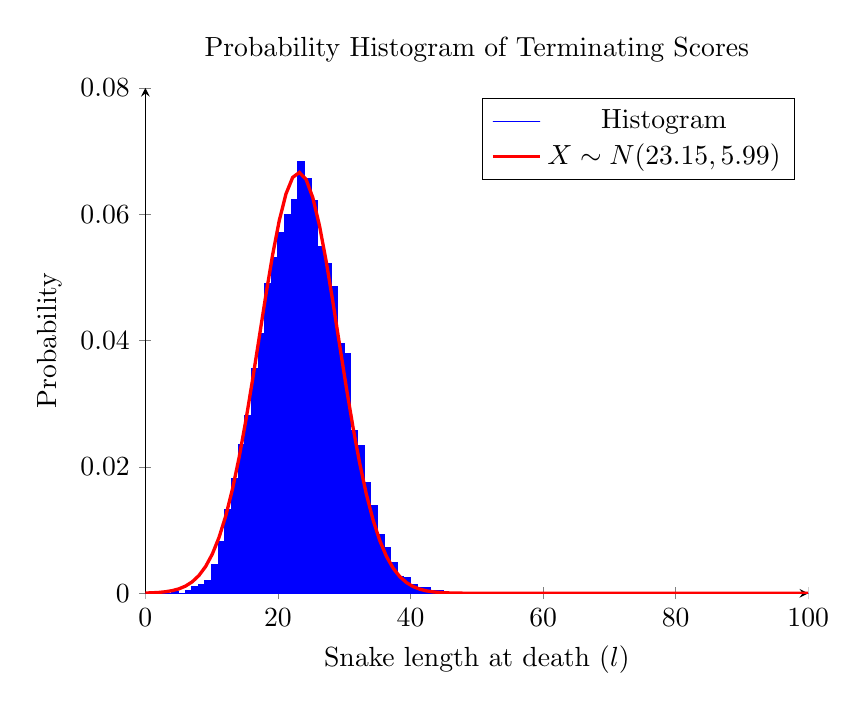
\begin{tikzpicture}
		\begin{axis}[
			title={Probability Histogram of Terminating Scores},
		    axis lines = left,
		    height=8cm,
		    xlabel = {Snake length at death ($l$)},
    		ylabel = {Probability},
    		xmin=0, xmax=100,
		    ymin=0, ymax=0.08,
		    yticklabel style={
	        	/pgf/number format/fixed,
    		    /pgf/number format/precision=5
			},
		]
		
			\addplot+[ybar interval,mark=no,color=blue,fill=blue] plot coordinates {(0, 0.0)(1, 0.0)(2, 0.0)(3, 0.0)(4, 0.0002)(5, 0.0)(6, 0.0004)(7, 0.001)(8, 0.0014)(9, 0.002)(10, 0.0045)(11, 0.0082)(12, 0.0132)(13, 0.0181)(14, 0.0236)(15, 0.0282)(16, 0.0356)(17, 0.0411)(18, 0.0491)(19, 0.0532)(20, 0.0571)(21, 0.06)(22, 0.0624)(23, 0.0684)(24, 0.0656)(25, 0.0621)(26, 0.0549)(27, 0.0522)(28, 0.0485)(29, 0.0396)(30, 0.0379)(31, 0.0257)(32, 0.0234)(33, 0.0176)(34, 0.0139)(35, 0.0093)(36, 0.0072)(37, 0.0048)(38, 0.0027)(39, 0.0025)(40, 0.0014)(41, 0.0009)(42, 0.0009)(43, 0.0004)(44, 0.0005)(45, 0.0001)(46, 0.0)(47, 0.0)(48, 0.0)(49, 0.0)(50, 0.0)(51, 0.0)(52, 0.0)(53, 0.0)(54, 0.0)(55, 0.0)(56, 0.0)(57, 0.0)(58, 0.0)(59, 0.0)(60, 0.0)(61, 0.0)(62, 0.0)(63, 0.0)(64, 0.0)(65, 0.0)(66, 0.0)(67, 0.0)(68, 0.0)(69, 0.0)(70, 0.0)(71, 0.0)(72, 0.0)(73, 0.0)(74, 0.0)(75, 0.0)(76, 0.0)(77, 0.0)(78, 0.0)(79, 0.0)(80, 0.0)(81, 0.0)(82, 0.0)(83, 0.0)(84, 0.0)(85, 0.0)(86, 0.0)(87, 0.0)(88, 0.0)(89, 0.0)(90, 0.0)(91, 0.0)(92, 0.0)(93, 0.0)(94, 0.0)(95, 0.0)(96, 0.0)(97, 0.0)(98, 0.0)(99, 0.0)(100, 0.0)};
			\addlegendentry{Histogram};
			
			\addplot [
				very thick,
		    	domain=0:100, 
	    		samples=100, 
		    	color=red,
			]
			{1/(5.99*(2*pi)^0.5)*e^(-((x-23.15)^2)/(2*5.99^2))};
			\addlegendentry{$X \sim N(23.15, 5.99)$};
		\end{axis}
	\end{tikzpicture}
	\caption{}
	\label{fig:bfs_sim_prob}
\end{figure}

As can be seen from this graph, the snake's dying lengths fit a normal distribution with mean $\mu = 23.15$ and standard deviation $\sigma = 5.99$. Note that because the dying length of a snake is a discrete variable being approximated by normal distribution, which is continuous, a continuity correction is needed. Rather the the height of the curve, it is the area under a continuous distribution that gives the probability of an event, so for an integer value $x$ from a set of discrete values including $\{\ldots, x-1, x, x+1, \ldots\}$, $P(X=x)$ can be approximated to $P(x-0.5 < X < x+0.5)$ \cite{wilson2011}. The halfway points are the boundaries of the bars that represent the area under the curve for the discrete value $x$.

For adding this probabilistic model to $T(l_s)$, we will find the probability of the snake being dead by a certain length. If this probability is very high, then it can be concluded that it is not favourable to continue using the BFS approach beyond this length, and the autonomous agent should switch to the Hamiltonian cycle approach. Using $e(l)$ to represent the probability that the snake will be dead (and the game will end) at length $l$, we have:
\begin{equation}
e(l) = P(0 < X < l + 0.5)
\end{equation}

\subsection{Optimization}

Finally, we can incorporate $e(l)$ into $T(l_s)$. For a constant $k$, we can now write $T(l_s)$ as:
\begin{equation}
T(l_s) = ke(l_s) + 0.4426l_{s}\ln(l_{s}) + \frac{1}{4}l_{s}^2 - 44.0429l_{s} + 2500
\end{equation}
The concept behind this equation is to penalize waiting longer to switch between approaches. The purpose of $T(l_s)$ was to model the number of total moves taken to beat the game by switching between the approaches at $l_s$, but since $e(l)$ grows at longer lengths as the probability of the snake dying by the BFS agent will increase the longer it gets, a "penalty" move count is added to $T(l_s)$. This will shift the local minimum of the graph towards a shorter switch length and will thus ensure that the switch length is not computed such that the snake will already be dead due to the BFS agent.

Since $0 \leq e(l) \leq 1$ whereas the total move counts are in the thousands, $e(l)$ is multiplied by a constant $k$. The bigger the value of $k$, the more the weight of the snake death penalty and the shorter the switch length of the snake. Referring back to experienced players who develop quick strategies to beat the game, their switch between the shortest path and the Hamiltonian cycle approach comes at a trade-off between finishing the game in a lower amount of time and dying early on. Essentially, $k$ is arbitrarily based on how "risky" a player wants to be in pursuit of a quicker win time. The graph shown in Figure \ref{fig:T_l_final_graph} below uses $k=700$. Using a GDC to compute the first local minimum of the final version of $T(l_s)$, we solve for the optimal length $l_s = 17.779$. Note this result is a real number, not an integer length. Thus, in practice, $\lfloor{l_s}\rfloor$ will be used as the switching point in the final agent as the safer option between $\lfloor{l_s}\rfloor$ and $\lceil{l_s}\rceil$ in terms of ensuring the snake's survival.

\begin{figure}[!h]
\centering
	\begin{tikzpicture}
		\begin{axis}[
		    axis lines = left,
		    xlabel = {$l_s$},
    		ylabel = {$T(l_s)$},
    		xmin=0, xmax=100,
		    ymin=0, ymax=2500,
		]

		\addplot gnuplot [very thick,mark=none,color=green,domain=0:100,samples=100] {350*erf(5.0*(20*x-463.0)/(599.0*sqrt(2))) + 0.4426*x*log(x) + 0.25*x^2 - 44.0429*x + 2850};
		\end{axis}
	\end{tikzpicture}
	\caption{Graphing $T(l_s)$}
	\label{fig:T_l_final_graph}
\end{figure}

\section{Evaluation}

\begin{figure}[!h]
\centering
	\begin{tabular}{ || c | c | c | c | c ||}
	\hline
	Approach & Dying Length & Total Moves & Win \% & Total Moves (Wins)\\
	\hline
	\hline
	Breadth-First Search & 22.89 & 164.77 & 0.00\% & —\\
	\hline		
	Hamiltonian Cycle & 100.00 & 2488.57 & 100.00\% & 2488.57\\
	\hline		
	Analytical ($l_s=17$) & 80.25 & 1454.93 & 77.61\% & 1871.94\\
	\hline		
	\end{tabular}
	\caption{Average dying length, move count and win \% for each approach, 1000 runs}
	\label{fig:approach_comparison}
\end{figure}

To determine the best approach, they can all be compared with respect to the data in Figure \ref{fig:approach_comparison} when they are run for 1000 trials. As expected from previous reflections, if Breadth-First Search was a flawless approach where the snake would never be trapped, it would have the least moves. The pure Hamiltonian cycle approach guaranteed a win, whereas the analytical approach, despite only winning 77.61\% of the time, takes 24.78\% less moves than the Hamiltonian cycle approach. The win rate and move count can be tuned arbitrarily by changing $k$.

The process of this investigation was successful at comprehensively mathematically modelling the $Snake$ game as well as generating a methodology for calculating the switch length for any $m$ and $n$ in the analytical approach. Transferring the logic to a computer program was also achieved. By contrast, one significant limitation was that experimental simulations were required to be conducted for finding a) coefficients for the logarithmic model of the move count function for the BFS approach and b) finding the correct $\mu$ and $\sigma$ values for the normal distribution of the probability function $e(l)$. Thus, while the applying the process undertaken to find $l_s$ for $m=n=10$ is robust, the dependence on large quantities of experimental data can become difficulty and resource-heavy to compute for much larger sizes of $m$ and $n$, making the overall approach not practical for the general case. Hence, a relevant extension could be to find a process not requiring experimental data. Additionally, $m$ and $n$ being constrained by the restriction of the Hamiltonian cycle limit the scope of the approaches used in the investigation. Another limitation is that by only exploring two base approaches, it cannot be conclusively determined that the overall approach is the most efficient way to win the game. For example, alternative path-finding algorithms other than BFS may be less prone to being trapped.

\section{Conclusion}

In conclusion, the most optimal algorithmic \textit{Snake} game agent was the one using both base approaches. The analytical approach was more efficient than the pure Hamiltonian cycle and more closely modelled how human players won the game in short times. The only consideration to make when choosing this approach is that for lower values of $k$, the win rate may not be very high. Through this exploration I learned many new concepts — namely graph theory — and applied concepts I was already familiar with to a real-life problem. This experience taught me that math can significantly help optimize and analyse real-world problems and the theory I used in this investigation are key for many applications I use daily, such as Google Maps.

\pagebreak
\begin{thebibliography}{9}
\bibitem{bose_howat2015}
Bose, Prosenjit, and John Howat. \textit{Depth-First Search and Breadth-First Search.} Discrete Mathematics Study Center. July 12, 2015. \\\texttt{https://cglab.ca/~discmath/graphs-applications.html}

\bibitem{easyspeezy2020}
EasySpeezy. \textit{He Thought I Couldn't Speedrun the Google Snake Game...} YouTube. November 15, 2020. \url{www.youtube.com/watch?v=O3bDZX0SAfk}

\bibitem{gadagkar2019}
Gadagkar, Shweta. \textit{Traversing Graphs in Discrete Math.} Study.com. September 16, 2018. \\\url{https://study.com/academy/lesson/coloring-traversing-graphs-in-discrete-math.html}

\bibitem{galvin2009} 
Galvin, David. \textit{Discrete Mathematics, Spring 2009 Graph Theory Notation.} March 4, 2009. \url{https://www3.nd.edu/~dgalvin1/60610/60610_S09/60610graphnotation.pdf}

\bibitem{liu2019}
Liu, Chuyang. \textit{Algorithms.} GitHub, November 18, 2019. \\\url{https://github.com/chuyangliu/snake/blob/master/docs/algorithms.md}

\bibitem{mitchell2019}
Mitchell, John. \textit{Hamiltonian Cycle Is NP-Complete.} Rensselaer Polytechnic Institute. February 2, 2019. \\\url{http://eaton.math.rpi.edu/faculty/Mitchell/courses/matp6620/notesMATP6620/lecture06/06A_hamiltoniancycle.pdf}

\bibitem{rahman2005}
M. Sohel Rahman, and M. Kaykobad. \textit{On Hamiltonian cycles and Hamiltonian paths.} Information Processing Letters 94, no.1 (2005): 37-41.

\bibitem{wilson2011}
Wilson, Steven. \textit{Almost Normal Distributions with Discrete Data.} Milefoot.com. September 4, 2011. \url{http://www.milefoot.com/math/stat/pdfc-normaldisc.htm}

\bibitem{zagaran2018}
Zagaran. \textit{Hamilton Paths/Cycles in Grid Graphs.} Mathematics Stack Exchange. August 31, 2018. \\\url{https://math.stackexchange.com/questions/1699203/hamilton-paths-cycles-in-grid-graphs}
\end{thebibliography}
\pagebreak
\appendix
\section{C++ Code}\label{sec:appendix_code}

\begin{figure}[!h]
\centering
\begin{lstlisting}
vector<Node> shortest_path(Node des) {
    queue<vector<Node> > q{{snake.back()}};
    vis.clear();
    for (Node u : snake)
      vis[u] = 1;
    vis[des] = 0;
    
    while (!q.empty()) {
      vector<Node> path = q.front();
      q.pop();
     
      if (path.back() == des)
        return path;
        
      for (Node u : path.back().adj()) {
        if (is_valid(u) && !vis[u]) {
          vis[u] = 1;
          vector<Node> new_path(path);
          new_path.push_back(u);
          q.push(new_path);
        }
      }
    }
    return {};
}
\end{lstlisting}
\caption{Code for performing a \textbf{Breadth-First Search}.}
\label{fig:bfs_code}
\end{figure}

\begin{figure}[!h]
\begin{lstlisting}
void build_cycle() {
    cycle.clear();
    vector<Node> path_dir = longest_path(snake[0]), snake_path = dir_path(snake);
    for (Node u : snake_path)
      path_dir.push_back(u);
    Node cur = snake.back();
    for (Node u : path_dir) {
      cycle[cur] = u;
      cur = cur + u;
    }
    cycle_size = path_dir.size();
}
\end{lstlisting}
\caption{Code for generating a \textbf{Hamiltonian Cycle} (heuristic) \cite{liu2019}}
\label{fig:cycle_code}
\end{figure}

\end{document}